% LaTeX Template for Project Report, Version 1.0
% (Abstracted for a Value Education Project Report at NIT Calicut but can be
% modified easily to use for other reports also.)
%
% Released under Creative Commons Attribution license (CC-BY)
%
% Created by: Kartik Singhal
% BTech CSE Batch of 2009-13
% NIT Calicut
% Contact Info: kartiksinghal@gmail.com
%
% It is advisable to learn the basics of LaTeX before using this template.
% A good resource to start with is http://en.wikibooks.org/wiki/LaTeX/
%
% All template fields are marked with a pair of angular brackets e.g. <title here>
% except for the ones defining citation names in ref.tex.
%
% Empty space after chapter/section/subsection titles can be used to insert text.
%
% Just compile this file using pdflatex after making all required changes.

\documentclass[12pt,a4paper]{report}
\usepackage[pdftex]{graphicx} %for embedding images
\usepackage{url} %for proper url entries
\usepackage[bookmarks, colorlinks=false, pdfborder={0 0 0}, pdftitle={A Food Review App for iPhone}, pdfauthor={Xinjiang Shao}, pdfsubject={UIC Project Report}, pdfkeywords={iOS, Foodie, Social, Location, Review}]{hyperref} %for creating links in the pdf version and other additional pdf attributes, no effect on the printed document
\usepackage[final]{pdfpages} %for embedding another pdf, remove if not required
\usepackage{figsize}

\begin{document}
\renewcommand\bibname{References} %Renames "Bibliography" to "References" on ref page

%include other pages
\begin{titlepage}

\begin{center}

\textup{\large A report on}\\[1.0cm]

% Title
\uppercase{\Large \textbf {Fancy Foodie : A Food Review App for iPhone}}\\[3.0cm]

% Done by
\normalsize Done by \\
\begin{table}[h]
\centering
\begin{tabular}{lr}\hline \\
Full Name & Xinjiang Shao \\ 
UIN & 675469866 \\ \\ \hline
\\
Advisor & Jakob Eriksson \\
Secondary Committee & Ugo Buy \\ \\ \hline 
\end{tabular}
\end{table}

\vfill

% Bottom of the page

\includegraphics[width=0.60\textwidth]{./uic-logo}\\[1cm]
\LARGE{Department of Computer Science}\\
\normalsize
\textsc{University of Illinois at Chicago}\\
%Calicut, Kerala 673 601 \\
\vspace{0.5cm}
Spring 2013

\end{center}

\end{titlepage}

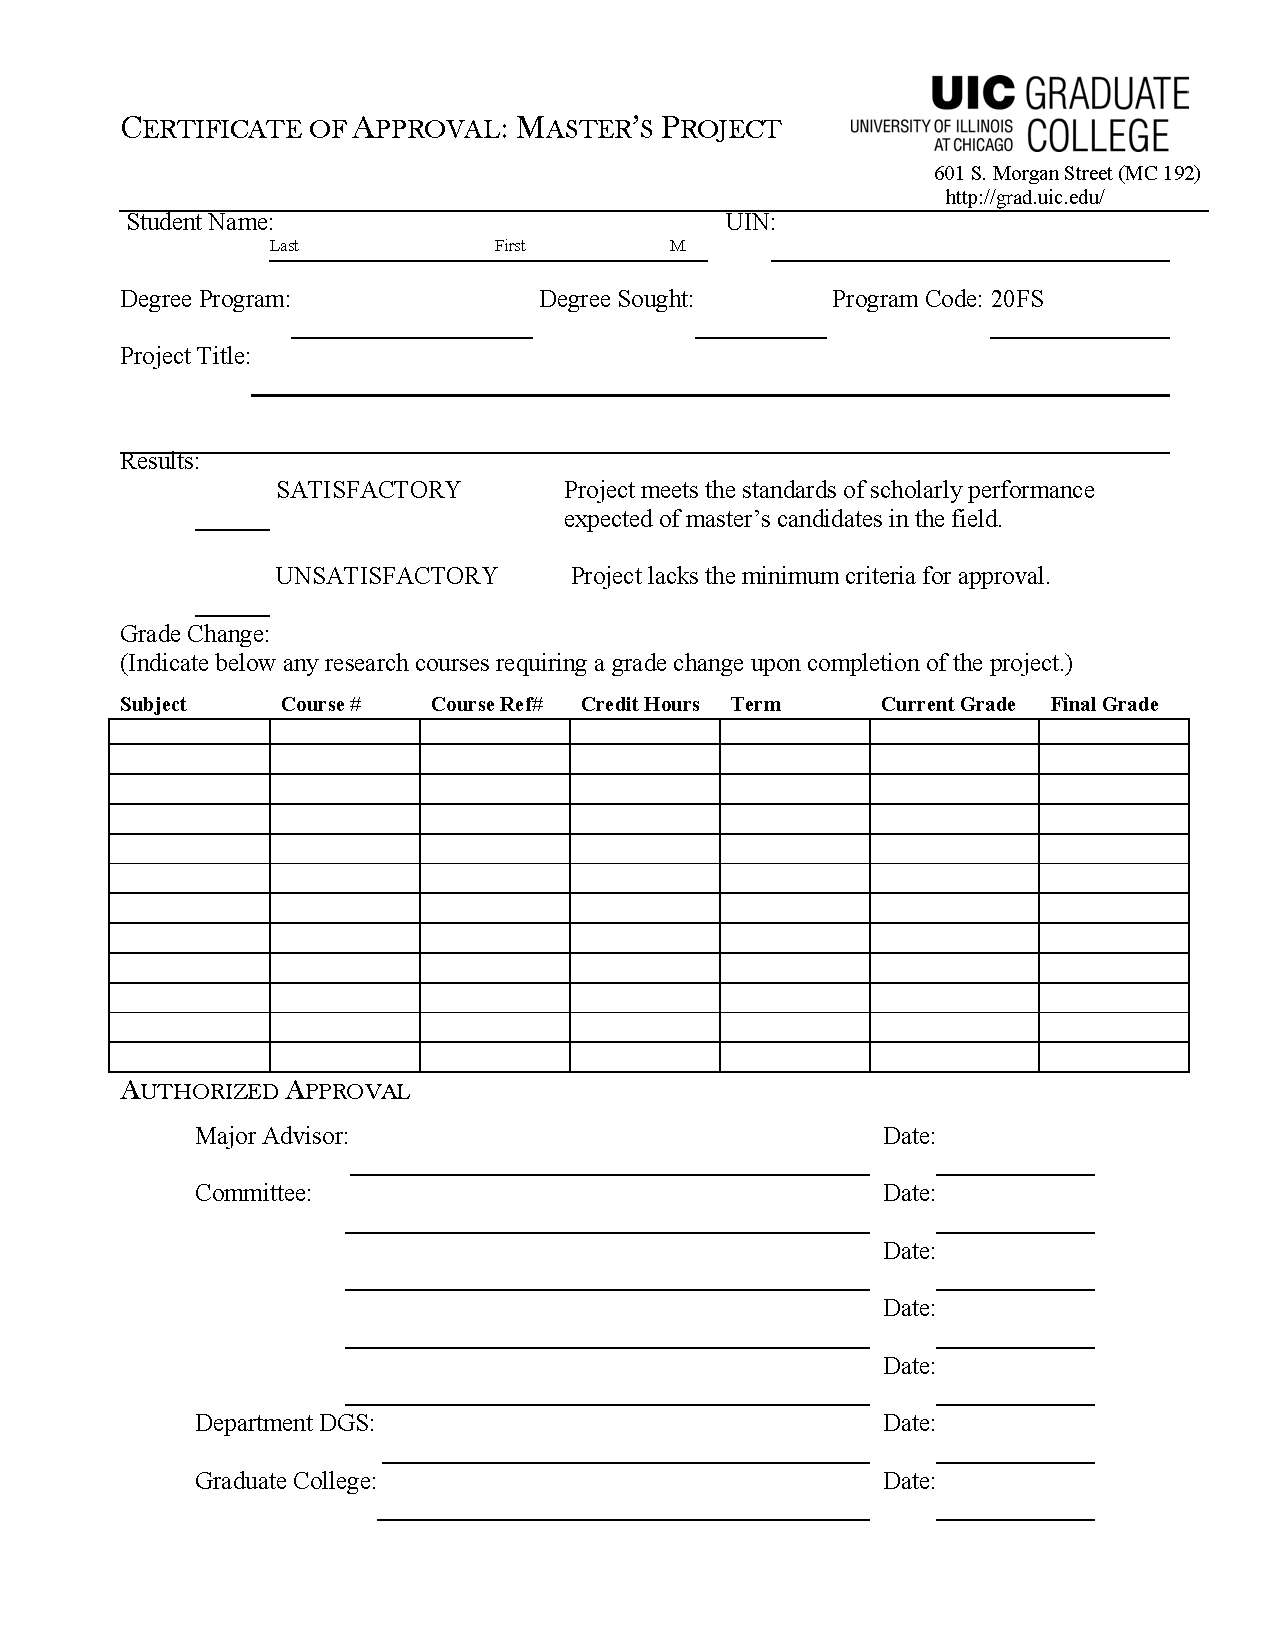
\includepdf{./CertificateofApprovalMAproject.pdf}
\vspace{2in}
\begin{abstract}

Food review is become trendy among young people since smart phone get more and more popular. However, not many tools available for people to review a cuisine and publish their comment to social media conveniently in the market. This project is meant to develop an iOS App called \emph{Fancy Foodie} that can take picture of food, attach meta data such as location, rate, comment, date, tags to the picture and sharing with friends via social media including Facebook, Twitter, Weibo etc.. The App also provides ways to search events by address and review statistic of all events. 

\end{abstract} 


\pagenumbering{roman} %numbering before main content starts
\tableofcontents
\listoffigures

\newpage
\pagenumbering{arabic} %reset numbering to normal for the main content

\chapter{Introduction}

Mobile Apps are making our life more and more interesting than ever before. A lot of young people love to take photo with their smart phone, making comments to it and sharing with their friend about what they had done. I personally find it would be useful if there is a tool for anyone to create food event and share with friends. \\


This project is a food review application called ``Fancy Foodie'' for iOS. The particular aim of the project is to be able to review food and sharing food event with friends. Before you start eating, the user would take a picture of the food they are going to eat and give some basic information about location, tags, date etc. Tags are used to describe the type of the food such as ``Chinese, Bun'' or ``Tea, Classic, Jasmine Green''. After finish eating, the user would make comments of the food. This application also lets user search nearby location or location defined by user, which will show a list of pins on the map where the user had been there before, to decide what the user want to eat. When the user saves a food event, he or she may also share the review and foodie's photo to Facebook or Twitter or to an email address. For user to see the history records, the application also provide a way to view statistics data such as how many places the user has been, how the rates are, how many tags the user used etc. ?\\


Currently, various of apps related to foodie are available in apple's app store. But most of them focused on the whole store/restaurant review. This could be inaccurate sometimes because you might just hate one dish. And there are also a few recipe-related apps. But the project want to have a better tool to publish what you eat instead of how that dish is made. \\ 


\chapter{Background}
\section{Motivation} % (fold)
\label{sec:motivation}

Seeking for places to eat is a thing in my genuine. I always want to keep track of my food adventures so that next time I could have better sense of what kind of courses I should order. I could also give recommendations to my friends about the adventures. Luckily, it turns out that I am not the only one want to do such kind of thing. A few of my friends tells that people nowadays love to take photos of the food before they eat, and post their photos to all kinds of social media such as Facebook, Twitter, Weibo (Chinese Twitter) etc.. Especially asian students have really strong motivation to take pictures of food when they eat. \\

After searching the apps available in apple app store, I didn't find any suitable choice for my need. So I came up with an idea that I need to make best use of skills and build a good app for people who like to explore food world with friends. 
\newpage

% section motivation (end)
\section{Restaurants Review Apps} % (fold)
\label{sec:current_review_apps}

\subsection{Yelp} % (fold)
\label{sub:yelp}

Yelp is used by tremendous people to get rate of restaurants in order to pick a place to eat. The searching filter for Yelp app is really good since they have a very rich database of different kinds of restaurants as well as different reviews from many people. The app provide a way to check with map and give direction the restaurant which is helpful for people to find the place. On the other hand, since they have a really large database, it is not easy to find what exactly you want to go. And most of the reviews are from people you don't know, it is highly possible that the taste of the people might be different from yours. Let alone there are people paid to make fake good reviews or bad reviews for some restaurants. \\

In this app, you're not using this looking for suggestions of where you're going to eat, but you need to get suggestions from your social media where your friends published restaurants reviews. In this way, fake reviews will be avoided. \\
% subsection yelp (end)
\newpage
% section current_review_apps (end)
\section{Recipe Related Apps} % (fold)
\label{awx:receipe_related_apps}
%some text\cite{citation-1-name-here}, some more text
\subsection{Evernote Food} % (fold)
\label{sub:evernote_food}

Food app from Evernote did a good job showing the meals. The user interface is really friendly. Adding tags to the meal is easy and choosing place information is convenient in Food.  The app also provided functionality to add a cuisine recipe as well. But people likes to take pictures of their food not always into making food. So in our project, we won't do any recipe recording.

% subsection evernote_food (end)
% section receipe_related_apps (end)





\chapter{Project Design}

\section{System Requirement} % (fold)
\label{sec:system_requirement}

\begin{itemize}
\item Operating System: iOS 6
\item Compile with Automatic Reference Counting (ARC)
\item Hardware Used: iPhone 5 and iPod Touch 4th Generation
\end{itemize}
 
% section system_requirement (end)
\newpage

\section{Design Philosophy} % (fold)
\label{sec:design_pholosiphy}

\subsection{Singleton Design Pattern} % (fold)
\label{sub:singleton_design_pattern}

	Design Pattern is used in this project. In software engineering, the Singleton Pattern arms at creating the instance of a class only one time so that we don't need to create twice. It is especially useful when you need to use a method of the class while the class is just a toolkit for you. In this project, we could this pattern to create a Settings instance in order to keep Settings globally shared inside of the app. There are a bunch of other places use this pattern as well, such as NearbyVenueController, LocationManager etc. \\
	
% subsection singleton_design_pattern (end)

\subsection{Model-View-Controller} % (fold)
\label{sub:model_view_controller}

	Another popular design philosophy in software engineering field is Model-View-Controller. This separate each parts so that we could focus on one thing instead of all together. We could call it as a divide and conquer method. The benefit to use it is that if we changed one Controller function, sometimes we don't need to update the view for it. It is a time and life saver for app designing. \\
	
% subsection model_view_controller (end)
\newpage
\section{Architecture} % (fold)
\label{sec:architecture}

	Figure~\ref{fig:storyboard} shows main views in storyboard. In this project, we build it as a tab based application. Five tabs are created for different purpose. Home tab plays as a guide to create a foodie event; Foodie list tab shows all the events created before; Statistics tab shows all aggregated data; Searching tab is used to show all past events and searching by address to find the events locations; Setting tab is for configurations.
	
\begin{figure}
	\centering
    \SetFigLayout[5]{1}{1}
    {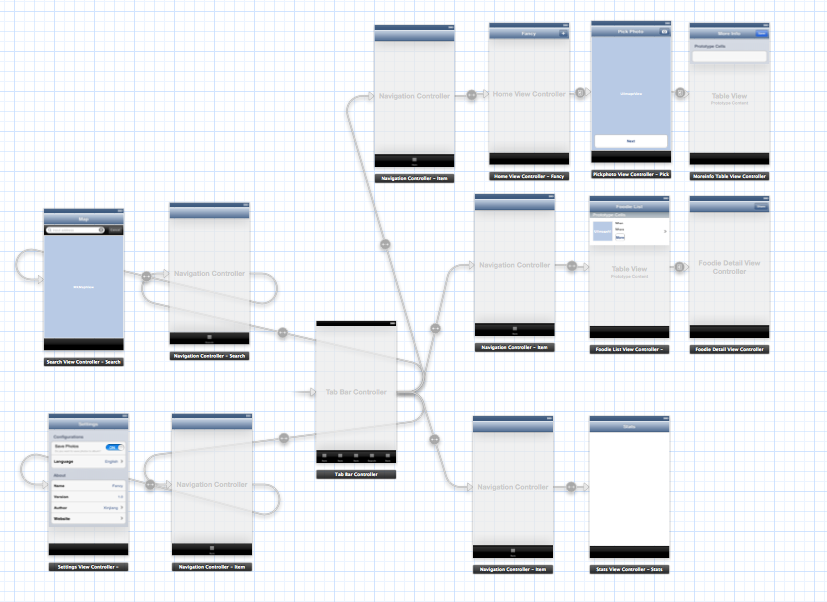
\includegraphics[%
    width=\figwidth, totalheight=\figheight, keepaspectratio]{./screenshots/storyboard-full.png}}
    \caption{Storyboard of Fancy Foodie}
	\label{fig:storyboard}
\end{figure}
% section architecture (end)
% section design_pholosiphy (end)




\chapter{Implementation}

\section{Data Model} % (fold)

\subsection{Database Schema} % (fold)
\label{sub:database_schema}

	In this project, we used three table for storing all the information from users. As Figure~\ref{fig:data-schema} shows, Events is the main table in the app. It provides fields ``address'', ``comment'', ``creationDate'', ``latitude'', ``longitude'', ``locationName'', ``rate'', ``thumbnail'', ``photoBlob'' and ``tags''. ``address'' field is used when user didn't find their ``locationName'' in location List fetching from Foursquare API v2. ``Latitude'' and ``longitude'' is used for adding annotations in Map View. A 80*80 resolution thumbnail is stored for each event in order to accelerate loading in food list table. \\ 
	
	``photoBlob'' has one to one relationship with ``photo'' in PhotoBlob table. Using a separate table should also help speeding up when we don't need to load photo while we still need to get the meta data of the event. \\
	
	Field ``tags'' has many to many relationship with ``photos'' in Tag table since one photo can labeled with many tags and one tag can relate to many photos.  
	
\label{sec:data_model}
\begin{figure}
	\centering
    \SetFigLayout{1}{1}
    {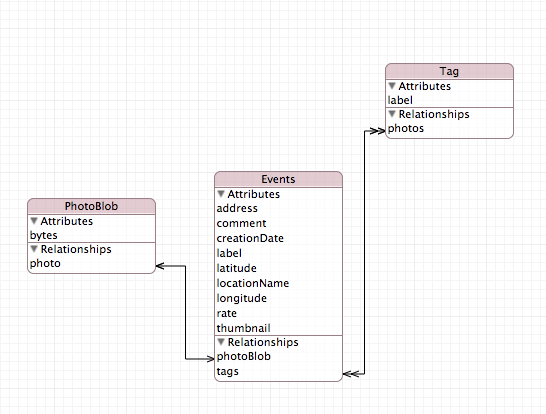
\includegraphics[%
    width=\figwidth, totalheight=\figheight, keepaspectratio]{./screenshots/database_schema.png}}
    \caption{Database Schema}
	\label{data-schema}
\end{figure}

% subsection database_schema (end)

\subsection{Settings Property List} % (fold)
\label{sub:settings_list}

	When developing iOS, we can also use another way to store data we need. Property List is used to store all information related to the app itself. For instance, using Property List to store App Display Name, App Version are commonly used in all apps for iPhone. \\
	
	``Fancy Foodie'' uses release number as main version string and git hash tag of the release as build string, so ``1.0 (build 98a9e84)'' is shown in Figure~\ref{fig:settings} which means that the main version number is 1.0 and build hash tag is 98a9e84. \\
	 
	 This app also use property list to store whether we need to save photo to album locally. If this option is enabled, the app will create a album  named ``Fancy Foodie Photos'' and put photos in this album as shown in Figure~\ref{fig:album}.
	 
 	 
% subsection settings_list (end)
% section data_model (end)
\newpage

\section{Workflow} % (fold)
\label{sec:work_overflow}

\subsection{Insert New Event} % (fold)
\label{sub:insert_new_event}

% subsection insert_new_event (end)

\subsection{Update Event} % (fold)
\label{sub:update_event}

% subsection update_event (end)

\subsection{Delete Event} % (fold)
\label{sub:delete_event}

% subsection delete_event (end)

\subsection{Searching Logic} % (fold)
\label{sub:searching_logic}

% subsection searching_logic (end)
\newpage
% section work_overflow (end)
\section{User Interface Design} % (fold)
\label{sec:user_interface_design}

\subsection{Home Tab} % (fold)
\label{sub:tabs}


\begin{figure}
    \centering
    \SetFigLayout{3}{3}
    \subfigure[Guide View]{
\includegraphics[width=\figwidth, totalheight=\figheight, keepaspectratio]{./screenshots/home.png}} \hfill
    \subfigure[Pick Action]{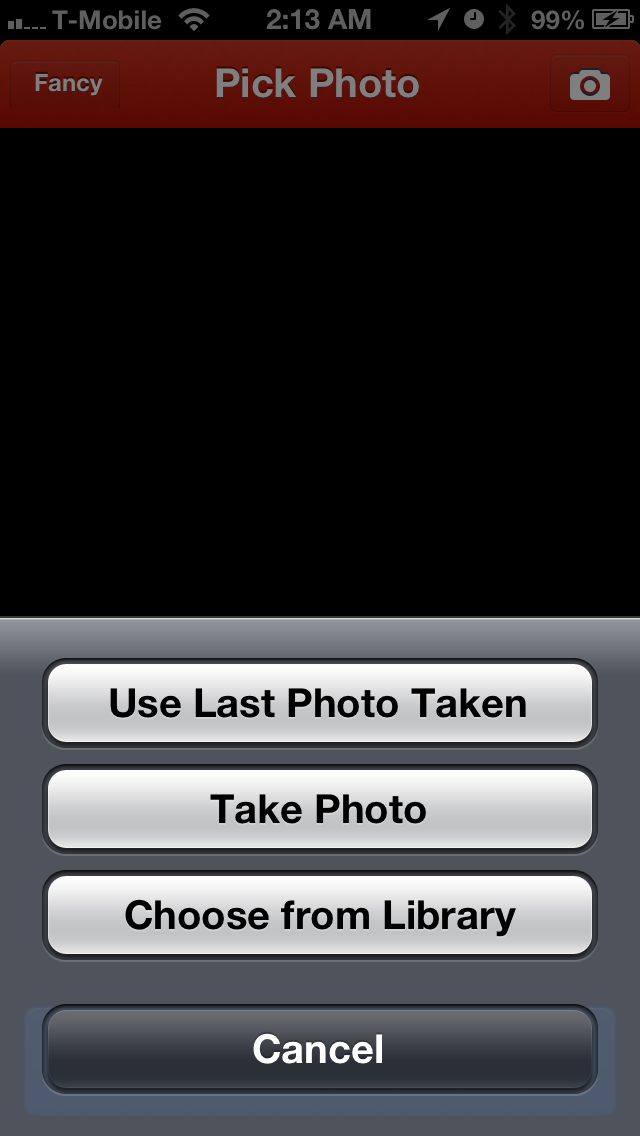
\includegraphics[width=\figwidth, totalheight=\figheight, keepaspectratio]{./screenshots/home-pickaction.png}} \hfill
	\subfigure[Move and Scale]{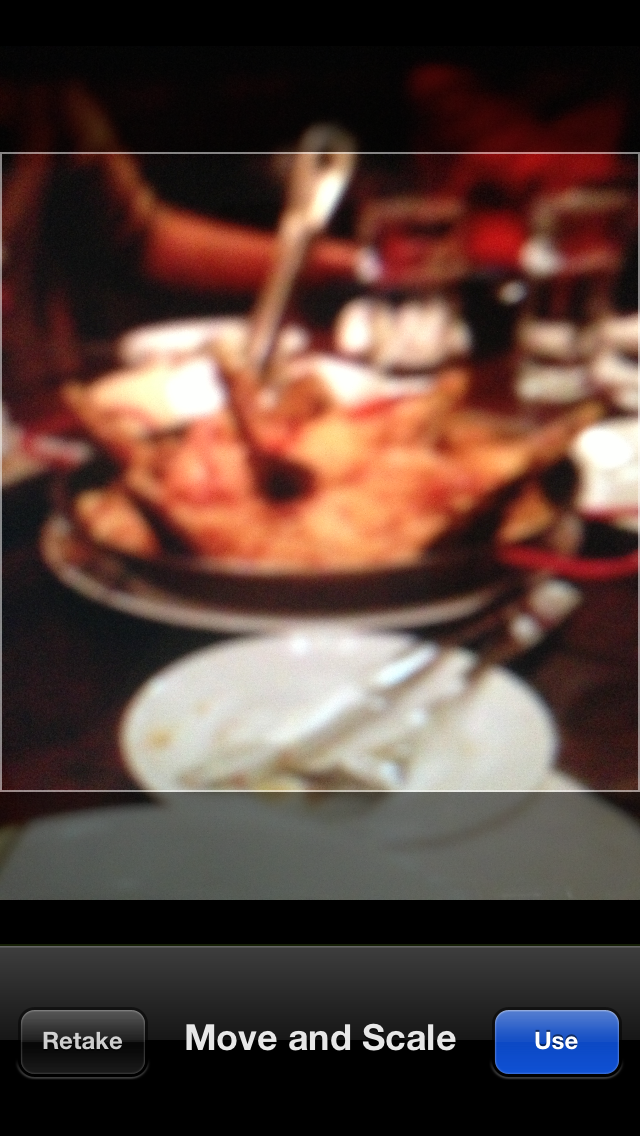
\includegraphics[width=\figwidth, totalheight=\figheight, keepaspectratio]{./screenshots/home-moveandscale.png}} \\ \hfill
    \subfigure[After Picking]{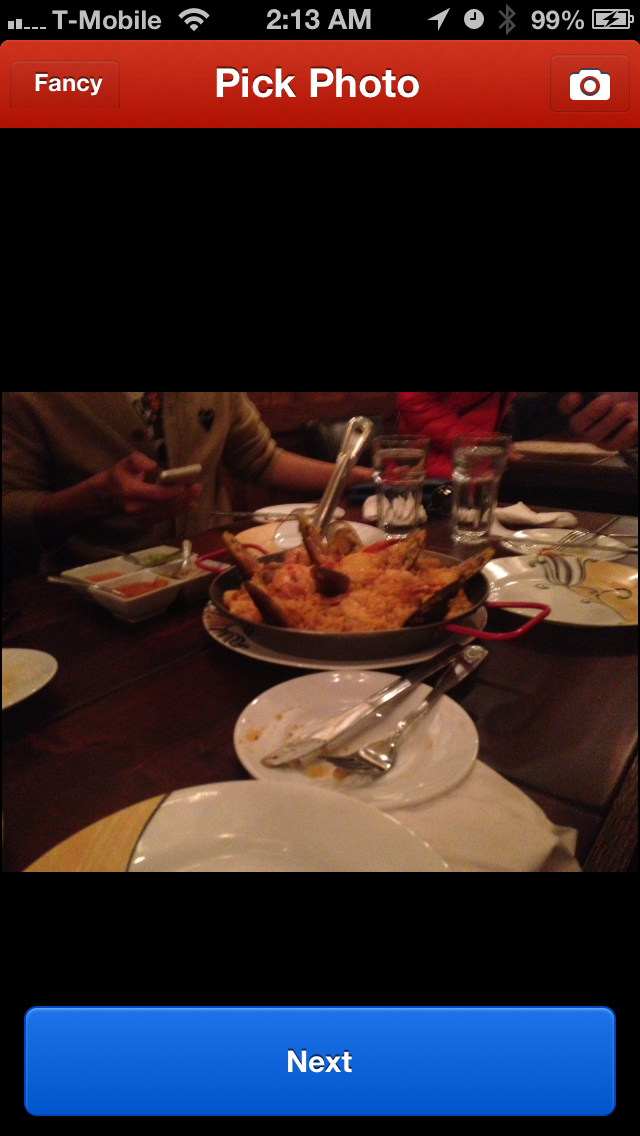
\includegraphics[width=\figwidth, totalheight=\figheight, keepaspectratio]{./screenshots/home-didpick.png}} \hfill
	\subfigure[Event Form]{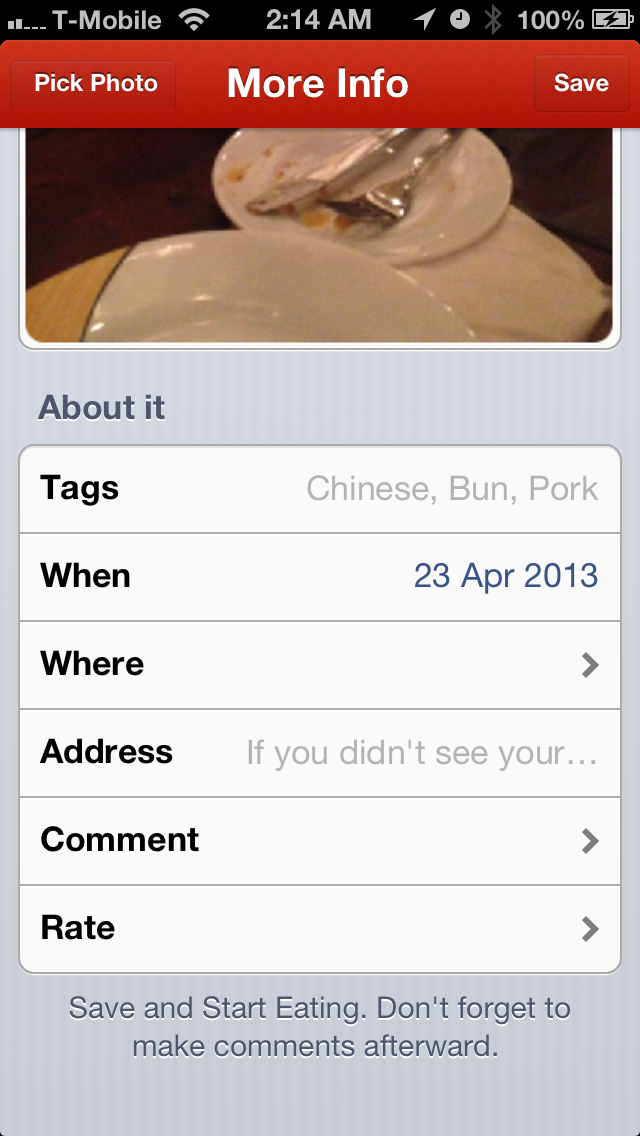
\includegraphics[width=\figwidth, totalheight=\figheight, keepaspectratio]{./screenshots/home-moreinfocontd.png}}   \hfill
    \subfigure[Date Picker]{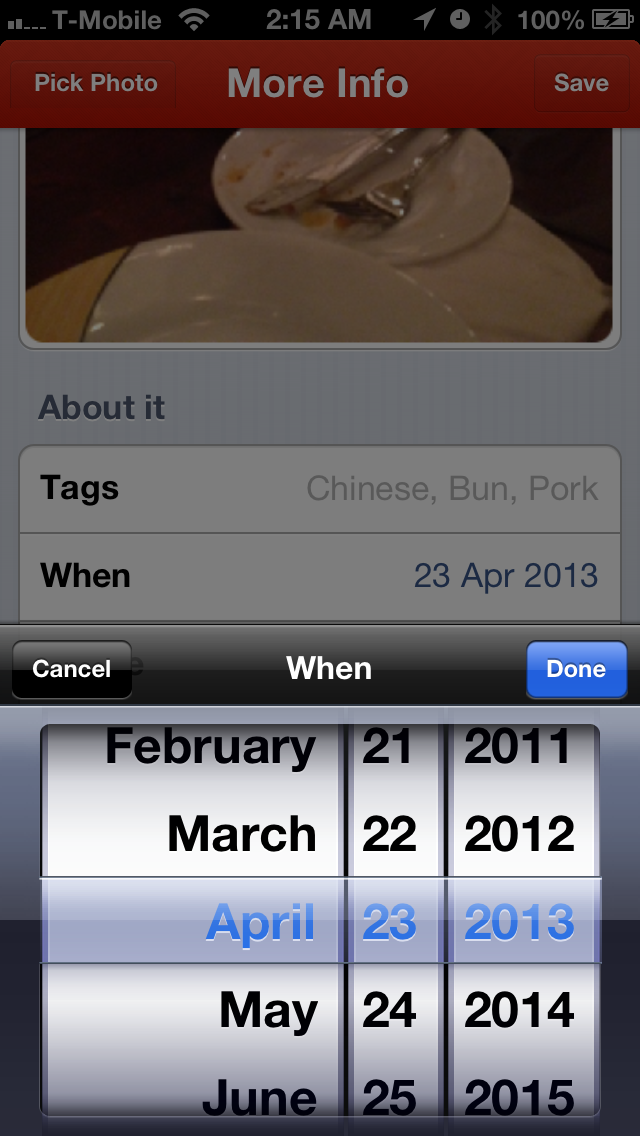
\includegraphics[width=\figwidth, totalheight=\figheight, keepaspectratio]{./screenshots/home-when.png}} \\ \hfill
    \subfigure[Location Picker]{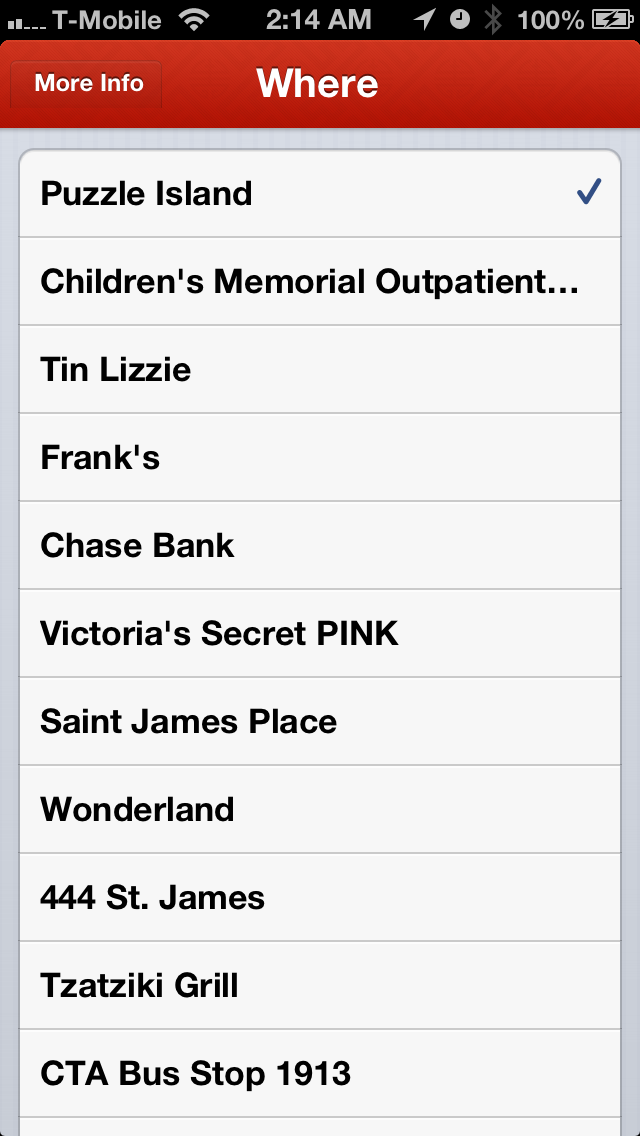
\includegraphics[width=\figwidth, totalheight=\figheight, keepaspectratio]{./screenshots/home-where.png}} \hfill
	\subfigure[Comment Editor]{
\includegraphics[width=\figwidth, totalheight=\figheight, keepaspectratio]{./screenshots/home-comment.png}}  \hfill
	\subfigure[Rate Picker]{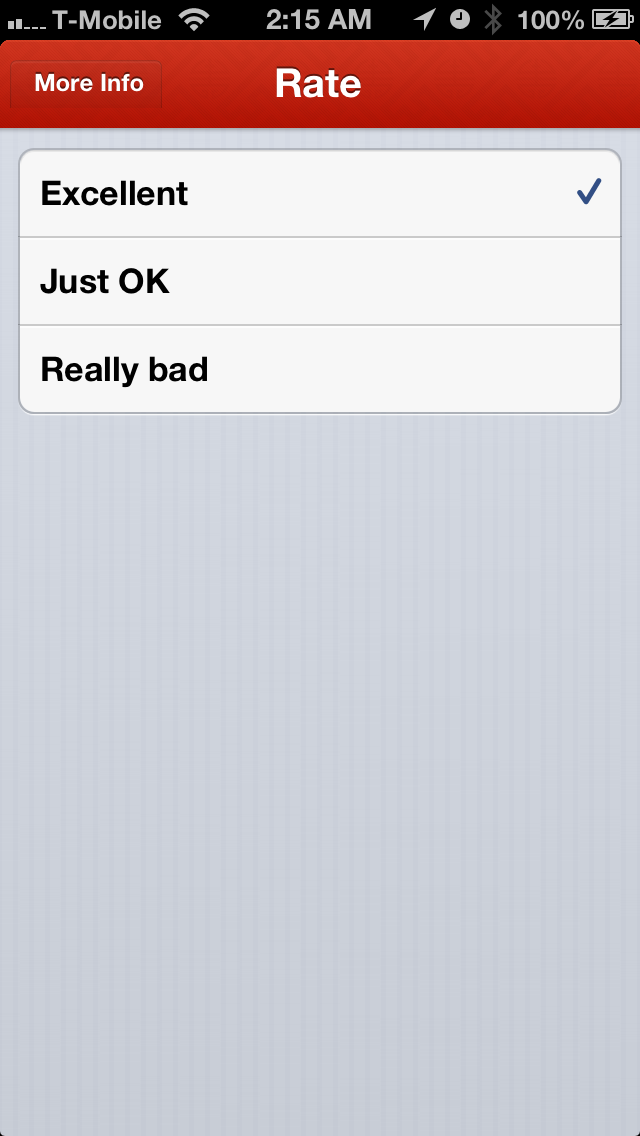
\includegraphics[width=\figwidth, totalheight=\figheight, keepaspectratio]{./screenshots/home-rate.png}} \hfill
	\caption{Home Tab View}
	\label{fig:hometab}
\end{figure}



% subsection tabs (end)

\subsection{Foodie List Tab} % (fold)
\label{sub:foodie_list_tab}

\begin{figure}
    \centering
    \SetFigLayout{2}{2}
    \subfigure[Foodie List]{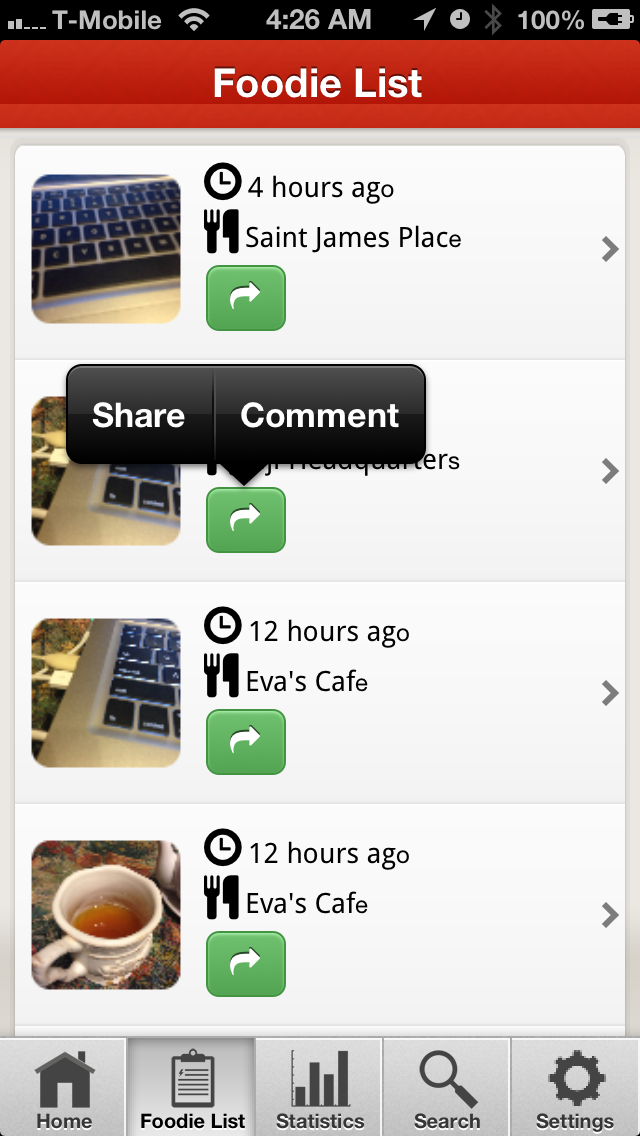
\includegraphics[width=\figwidth, totalheight=\figheight, keepaspectratio]{./screenshots/foodielist.png}} \hfill
	\subfigure[Sharing]{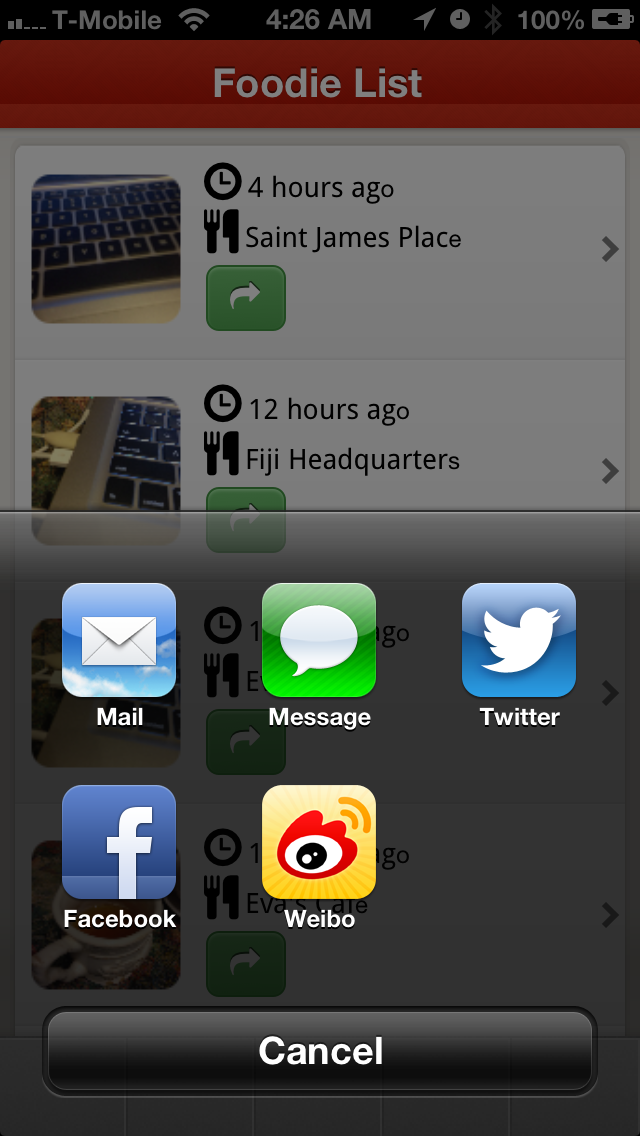
\includegraphics[width=\figwidth, totalheight=\figheight, keepaspectratio]{./screenshots/foodielist-share.png}} \hfill \\
	\subfigure[Detail View]{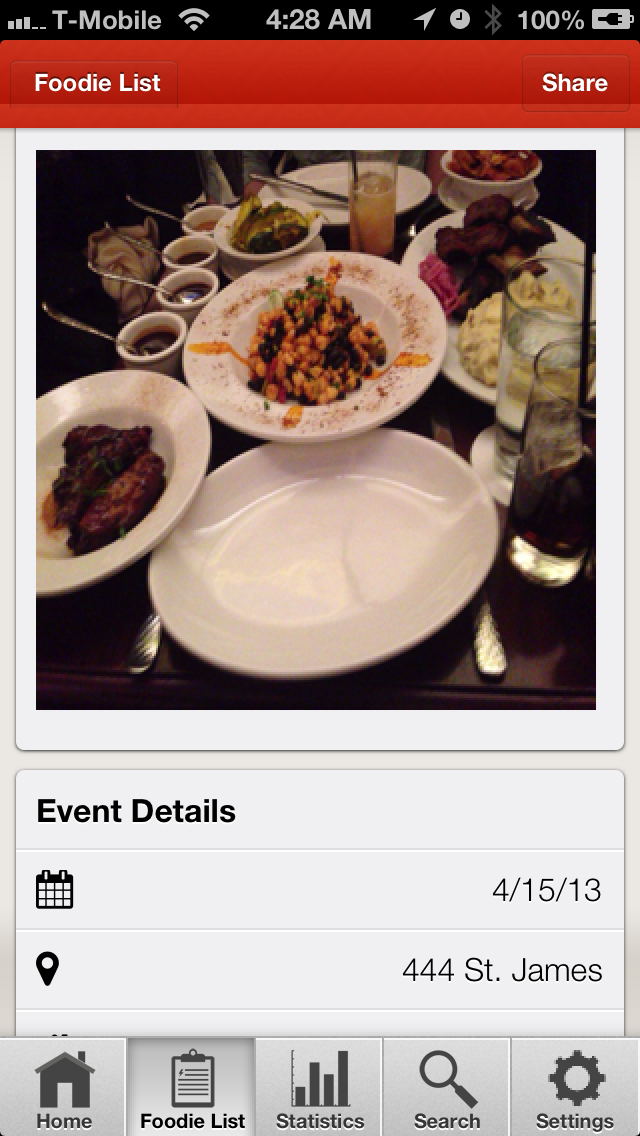
\includegraphics[width=\figwidth, totalheight=\figheight, keepaspectratio]{./screenshots/foodielist-detail.png}} \hfill
	\subfigure[Detail View Cont'd]{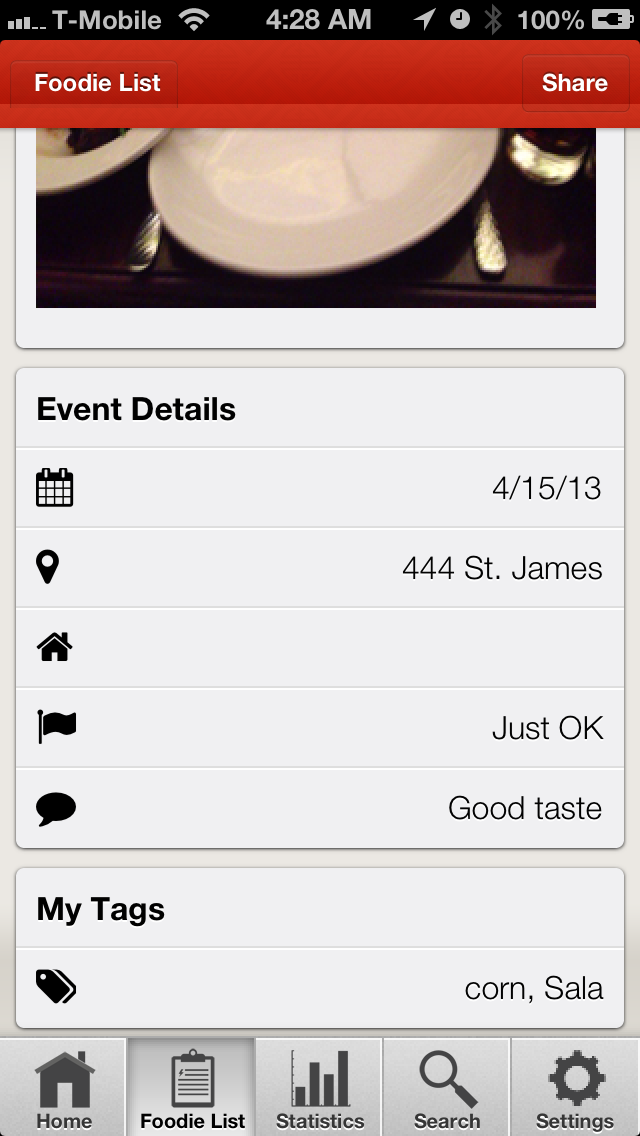
\includegraphics[width=\figwidth, totalheight=\figheight, keepaspectratio]{./screenshots/home-form-continued.png}} \hfill
	\caption{Foodie List Tab View}
	\label{fig:foodielisttab}
\end{figure}




% subsection foodie_list_tab (end)

\subsection{Stats Tab} % (fold)
\label{sub:stats_tab}

\begin{figure}
	\centering
    \SetFigLayout{1}{1}
    {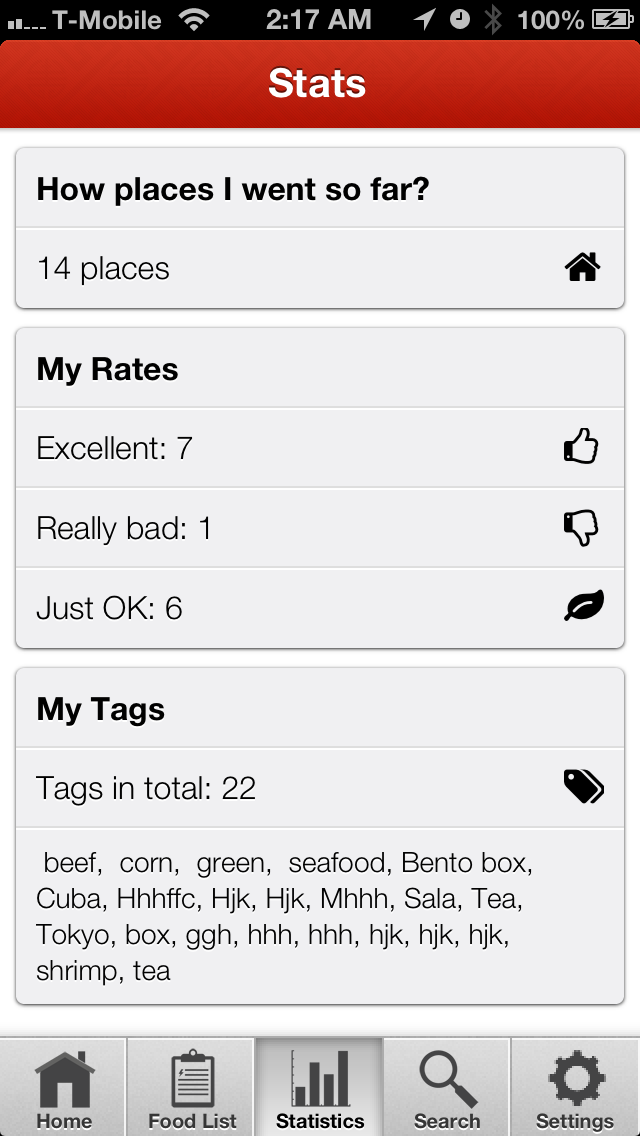
\includegraphics[%
    width=\figwidth, totalheight=\figheight, keepaspectratio]{./screenshots/stats.png}}
    \caption{Statistics Tab View}
\end{figure}

% subsection stats_tab (end)
\subsection{Map Tab} % (fold)
\label{sub:map_tab}

\begin{figure}
	\centering
    \SetFigLayout{1}{1}
    {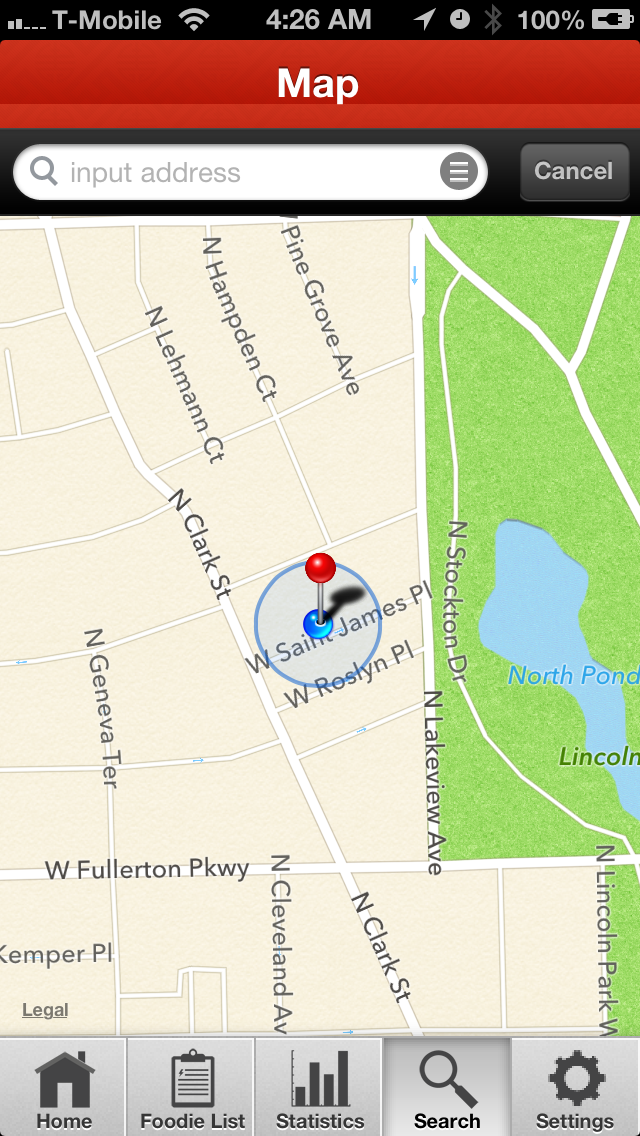
\includegraphics[%
    width=\figwidth, totalheight=\figheight, keepaspectratio]{./screenshots/map.png}}
    \caption{Map Tab View}
\end{figure}

% subsection map_tab (end)

\subsection{Setting Tab} % (fold)
\label{sub:setting_tab}

\begin{figure}
	\centering
    \SetFigLayout{1}{1}
    {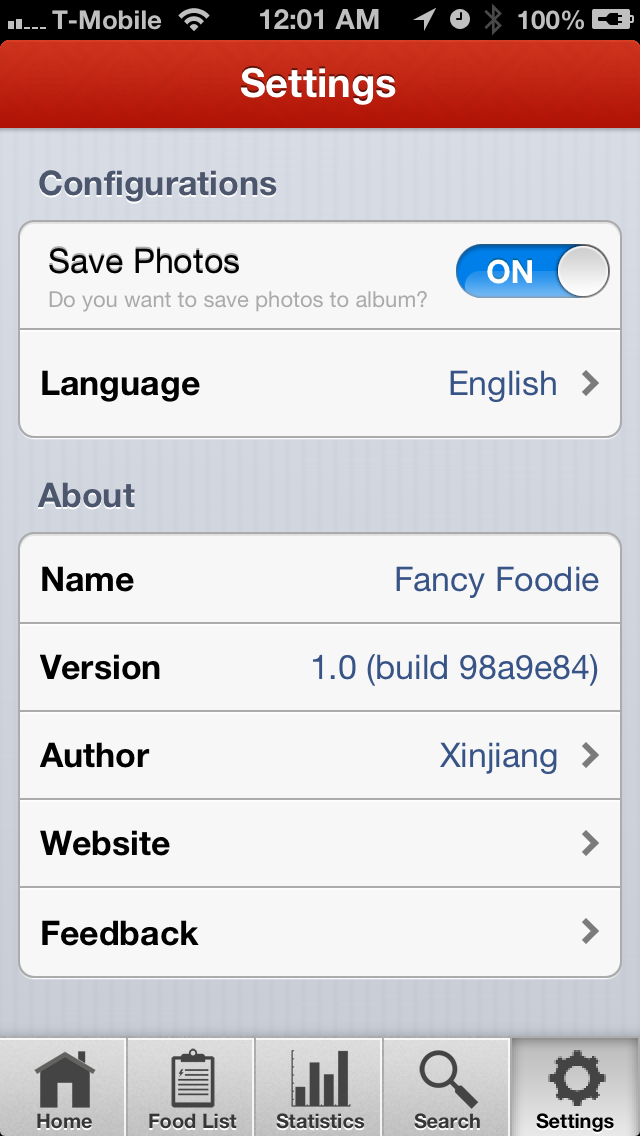
\includegraphics[%
    width=\figwidth, totalheight=\figheight, keepaspectratio]{./screenshots/settings.png}}
    \caption{Setting Tab View}
	\label{settings}
\end{figure}
\begin{figure}
	\centering
    \SetFigLayout{1}{1}
    {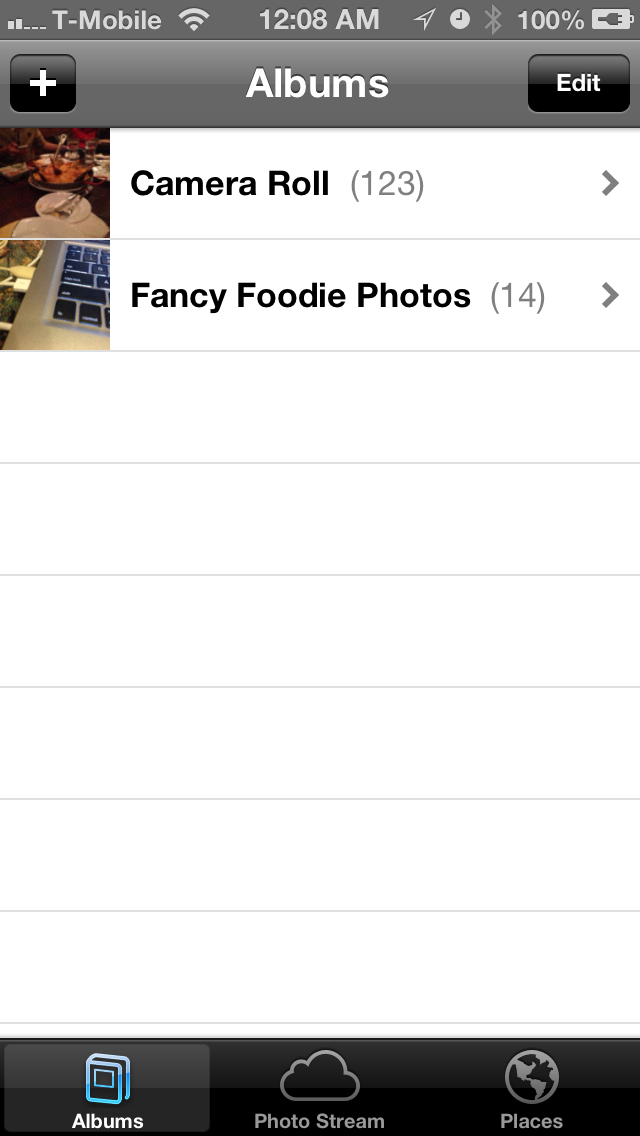
\includegraphics[%
    width=\figwidth, totalheight=\figheight, keepaspectratio]{./screenshots/settings-album.png}}
    \caption{Album View}
	\label{album}
\end{figure}
% subsection setting_tab (end)
% section user_interface_design (end)

\chapter{Future Work}

Yelp Intergation 

Centeral Database

Multi-languages

beta Test


\chapter{Conclusion}

This project is successfully finished in time with good functionalities overall. It could provide users to take picture of food they like and create tags, location information, rates, and comments to the food. At the time, it provides convenient methods for users to share those food with their friend by social media such as Facebook, Twitter, Weibo etc.. A map view and statistics view are created for users to have better understanding of their preferences. \\

There are still more features could be done in future. Since Yelp is a good resource of restaurant information, the app could pull more information from Yelp in order to give users more about the place they eat at. A central database is needed to making users communicate with each other such as making comments to friends food inside of the app. Chinese is my mother tongue, so I'm hoping to adding multi-language feature for the App. In this way, more people could be able to use the App. Last but not least, a larger pool of testers should be included in beta testing process.

\clearpage
\addcontentsline{toc}{chapter}{Acknowledgements}
\chapter*{Acknowledgments}
\vspace{1.0in}

I would like to thank open source community. Without them, I probably need much more time to finish this project. \\

I would also like to thank Jakob Eriksson and Ugo Buy. Prof. Eriksson gave me a lot of valuable suggestion for my project.  Prof. Buy also provided helpful suggestion on the report. Both Prof. Eriksson and Prof. Buy give a good evaluation of my work. \\

Special thanks to all my friends who made tremendous comments about my app and all my colleagues in EXACT Sports LLC who slow me down in the right way so that I can make the project better. \\

%{Xinjiang Shao}\\ 
\leavevmode
\\
\\
\\
\\
\\
Xinjiang Shao \\
{April 2013}\\
{University of Illinois at Chicago}\\
\newpage

\addcontentsline{toc}{chapter}{References}
\begin{thebibliography}{99}

\bibitem{citation-1-name-here}<Name of the reference here>,\ \url{<url here>}

\bibitem{citation-2-name-here}<Name of the reference here>,\ \url{<url here>}

\end{thebibliography}


\end{document}
